\chapter{Πειράματα και Αποτελέσματα}
\label{ch:experiments}
Η εκτέλεση όλων των πειραμάτων που παρουσιάζονται παρακάτω 
πραγματοποιήθηκε σε πόρους της Ιδρυματικής συστοιχίας του 
ΑΠΘ "Αριστοτέλης".
Το μοντέλο επεξεργαστή που χρησιμοποιήθηκε για τα πειράματα 
είναι \tl{Intel Xeon E5-2630 v4}.
Η υλοποίηση των αλγορίθμων έγινε στη γλώσσα \tl{"Julia Version
1.7.2"}. 


\section{Κόστος Υπολογισμού Απόστασης Στοιχείων}
\label{sec:geom_tests_cost}
Για τον προσδιορισμό του κόστους $C_v$ και $C_p$
της μετρικής κόστους της ενότητας \ref{sec:cost_metric}
θεωρήσαμε πως το κόστος υπολογισμού της τετραγωνική απόστασης
δύο σημείων είναι μονάδα.
Όλα τα υπόλοιπα κόστη, λοιπόν, υπολογίζονται σε σχέση με το 
κόστος σημείο-σημείο. 
Μετρήσαμε τον χρόνο υπολογισμού των τετραγωνικών αποστάσεων 
περίπου $210\times10^6$ σημείων, \tl{AABB}, ευθυγράμμων τμημάτων 
και τριγώνων και προέκυψε ο πίνακας \ref{tab:distance_rel_cost} 
με τα σχετικά κόστη. Επομένως, $C_v=23.5$, $C_p=385.7$.

\begin{table}[h]
    \centering
    \begin{tabular}{|c|c|}
        \hline 
        Υπολογισμός Απόστασης & Κόστος \\
        \hline
        Σημείο-Σημείο & $1$ \\
        \hline 
        AABB-AABB & $23.5$ \\
        \hline
        Ευθ. Τμήμα - Ευθ. Τμήμα & $129.8$ \\
        \hline
        Τρίγωνο-Τρίγωνο & $385.7$ \\
        \hline
    \end{tabular}
    \caption[]{Σχετικό κόστος υπολογισμού της απόστασης διαφόρων στοιχείων}
    \label{tab:distance_rel_cost}
\end{table}

\section{Κατασκευή Δεδομένων Ελέγχου}
Για την εκτέλεση των πειραμάτων κατασκευάσαμε διάφορα σενάρια.
Κάθε σενάριο αποτελείται από δύο αντικείμενα και για το κάθε 
αντικείμενο κατασκευάσαμε τριγωνικά πλέγματα με τρεις διαφορετικές 
αναλύσεις (διαφορετικό πλήθος τριγώνων).
Έτσι, για κάθε σενάριο εκτελούμε ερωτήματα εύρεσης της απόστασης 
των αντικειμένων για κάθε συνδυασμό ανάλυσης (σύνολο 9 μετρήσεις).
Έγινε προσπάθεια συμπερίληψης διάφορων περιπτώσεων, με αντικείμενα 
διαφόρων σχημάτων, διαστάσεων και προσανατολισμού.

Η λήψη των αντικειμένων που χρησιμοποιούνται σε αυτή την εργασία 
έγινε από το \tl{GrabCAD}\cite{GrabCAD} και το \tl{3D Content Central}
\cite{3dcontentcentral}. 
Τα αντικείμενα, αρχικά, ήταν σε μορφή \tl{\texttt{IGES}}, ενώ για τη 
δημιουργία των πλεγμάτων χρησιμοποιήθηκε το πρόγραμμα 
\tl{BETA CAE SYSTEMS - Ansa v21.0.0}.

% TODO: ADD PHOTOS OF EACH SCENARIO

\section{Χρόνος Κατασκευής του \tl{sKD-Tree}}
Στο σχήμα \ref{fig:build_time} παρουσιάζονται οι μετρήσεις του 
χρόνου κατασκευής του \tl{sKD-Tree} συναρτήσει του μεγέθους ενός 
τριγωνικού πλέγματος και του πλήθους των νημάτων (\tl{threads})
που χρησιμοποιήθηκαν.

\begin{figure}[h]
    \centering
    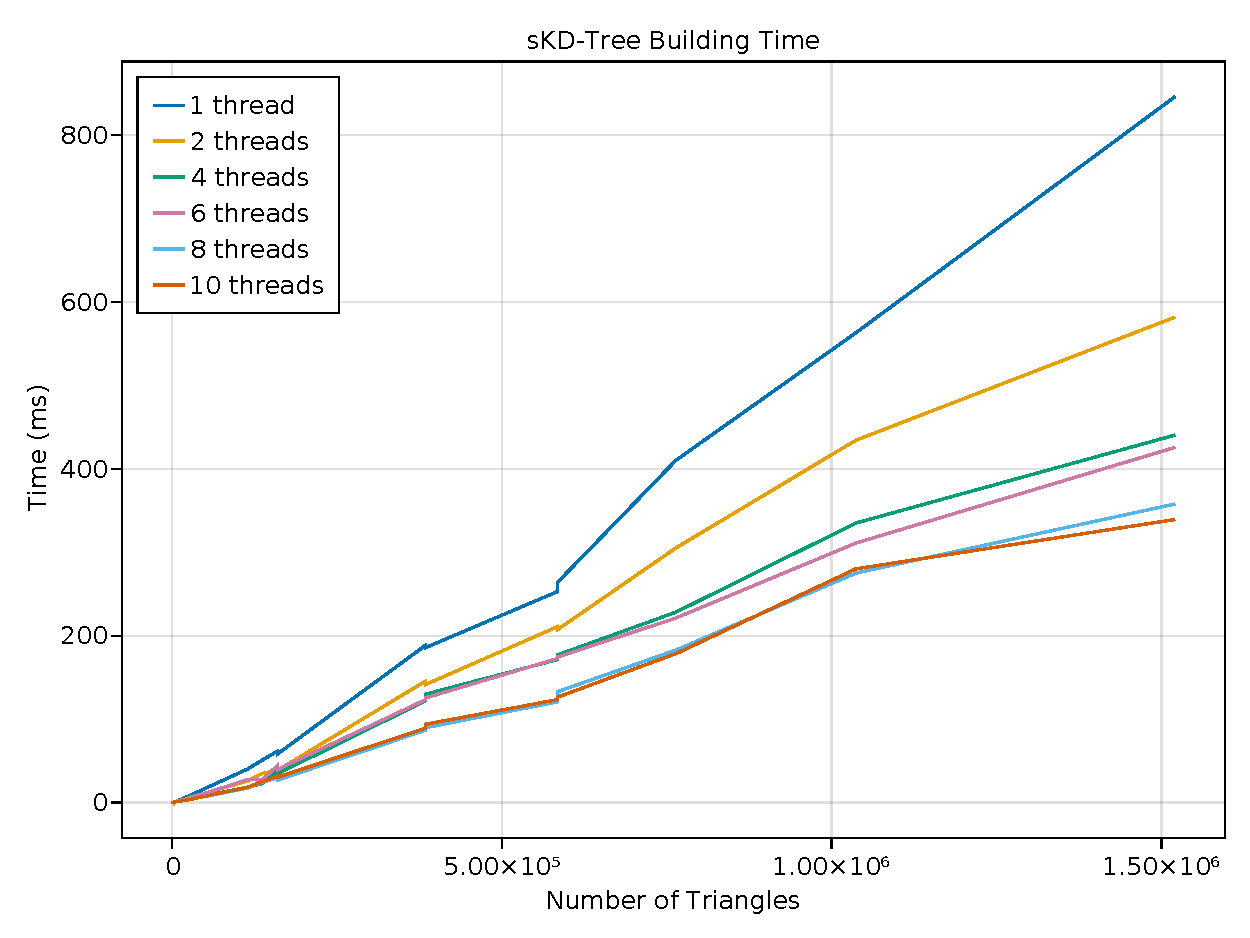
\includegraphics[width=0.6\textwidth]{build_time.pdf}
    \caption[Χρόνοι Κατασκευής του \tl{sKD-Tree}]{
        Χρόνος κατασκευής του \tl{sKD-Tree} συναρτήσει 
        του πλήθους των τριγώνων ενός πλέγματος.
    }
    \label{fig:build_time}
\end{figure}

\section{Εκτίμηση της Μετρικής Κόστους Αναζήτησης}

\section{Συνολικός Χρόνος Εκτέλεσης - Σύγκριση Αλγορίθμων}

\section{Επίδραση της Απόστασης }

% να προσθέσω ποσοστά χρόνου αναζήτησης/κατασκευής
\subsection{Δύο Αεροπλάνα}
\subsection{\tl{Scooby} με \tl{Stanford Bunny}}
\subsection{Δύο Ομοαξονικοί Κύλινδροι}
\subsection{Δύο Αεροπλάνα με Ανομοιόμορφο Πλέγμα}
